\subsection{Potencias en un sistema alimentado con corriente alterna}

   Se puede definir el concepto de \textbf{potencia}, como cantidad de energía eléctrica 
  entregada o absorbida por un elemento en un momento determinado, cuya unidad en el Sistema 
  Internacional de Unidades es el \textbf{watt} (\textbf{W}).

   En circuitos de corriente alterna (CA), se puede determinar 3 tipos de potencias:
   \textbf{activa}, \textbf{reactiva} y \textbf{aparente}.

  La potencia activa (\textbf{P}) también conocida como la \textit{potencia real}, es la que
  es consumida por cargas resistivas propias de un circuito, y es medida 
  en \textbf{watt} (\textbf{W}). La potencia reactiva (\textbf{Q}), es la potencia 
  intercambiada por cargas inductivas y/o capacitivas; su unidad de medida es 
  \textbf{volt-ampere reactivo} (\textbf{VAR}). Por último, la potencia aparente (\textbf{S}),
  es una combinación entre la potencia activa y la reactiva; su unidad de medida es 
  \textbf{volt-ampere } (\textbf{VA}).

  Estas potencias se relacionan entre sí de la siguiente manera. Partiendo de una señal

        \vspace{-15pt}  
        \begin{align}
            v(t)   &= V_m \sin(\omega t)\ [V] ~, \notag \\
            \intertext{que excita un circuito genérico que contiene una impedancia 
                        $Z = R + jX = |Z| \angle \varphi$,  se produce una corriente
                        eléctrica cuya forma es}
            i(t)   &= I_m  \sin(\omega t - \varphi)\ [A] \ , \notag \\
            \intertext{entonces, la potencia instantánea, asociada a la señal de 
                excitación, se obtiene mediante el producto de la tensión por la 
                corriente, dando como resultado}
            p(t)  &= [V_m \sin(\omega t)] 
            \cdot [I_m \sin(\omega t - \varphi)]\ [W]  ~.
                            \label{eqn:Winst}
         \end{align}

      
    Ahora, partiendo de la ecuación~(\ref{eqn:Winst}), la misma se la puede reescribir de la
    siguiente forma (mediante la identidad trigonométrica del \textit{seno de la resta})

        \vspace{-15pt}
         \begin{align}
            p(t)  &= V_m \sin(\omega t)\cdot [I_m \sin(\omega t) \cos(\varphi) - I_m \cos(\omega t) \sen(\varphi)]  \notag \\
            p(t)   &= [2 \sin^{2}(\omega t)]\cdot V I \cos(\varphi) - [2 \sin(\omega t) \cos(\omega t)]\cdot V I\sen(\varphi) ~.\notag \\
            \intertext{Luego, aplicando las identidades}
                  &2 \sin^{2}(\alpha)  = 1 - \cos(2\alpha) \hspace{20pt} ; \hspace{20pt} \sin(2\alpha) = 2 \sin(\alpha) \cos(\alpha) \ , \notag \\
            \intertext{finalmente queda la siguiente expresión}
            p(t)  &= [1- \cos(2 \omega t)]\cdot V I \cos(\varphi) - [\sin(2 \omega t)]\cdot V I \sin(\varphi) ~. 
         \end{align}

      De esta última expresión obtenida se observa que el primer término del segundo miembro
      de la ecuación, corresponde a la \textbf{potencia activa P} asociada a lo componentes
      resistivos de un sistema, mientras que el segundo término del mismo, corresponde a la 
      \textbf{potencia reactiva Q}, asociada a los componentes reactivos del mismo.

      Operando algebráicamente la última expresión obtenida, se obtiene la versión reducida
      de dichas potencias   

        \begin{equation}
            \boxed{P   = V I \cos(\alpha)~[W]}~.  \label{eqn:PotActTot}
        \end{equation}
        \begin{equation}
            \boxed{Q   = V I \cos(\alpha)~[VAR]}~. \label{eqn:PotReacTot}
        \end{equation}

      Por último, la \textbf{potencia aparente total} (\textbf{S}), se obtiene  sumando los aportes de
      las potencias activas y reactivas, y como estas mismas se realizan en cuadratura, entonces

        \begin{equation}
            S^{2} = P^{2} + Q^{2} \hspace{20pt} \therefore \hspace{20pt} \boxed{S = \sqrt{P^{2} + Q^{2}}~[VA]} ~. \label{eqn:PotApaTot}       
         \end{equation}


         \subsubsection{Obtención del triángulo de potencia mediante fasores}
            El cálculo de las potencias resistivas y reactivas se puede obtener de manera
            directa mediante el uso de fasores. A continuación, se deducen los cálculos
            necesarios para la obtención.
            Partiendo de una tensión descrita en fasores $\vec{V} = |\vec{V}| \angle \,  0^{\circ} $,
            excitando un circuito con una impedancia $ Z = |Z| \angle \pm \varphi \ $, se
            genera una corriente $\vec{I}  = \vec{|I|} \angle \mp   \varphi $~.

            La potencia activa total, como se vio en la sección anterior, se puede obtener 
            mediante la ecuación~(\ref{eqn:PotActTot}). La misma se puede reescribir en término de 
            fasores como el \textit{producto de sus módulos por el coseno del ángulo entre ellos}
               \begin{align}
                  P = \vec{|V|} \vec{|I|} \cos(\varphi) = V I \cos(\varphi)~. \notag
               \end{align}   

            \noindent La potencia reactiva total, como se vio en la sección anterior, se puede obtener 
            mediante ecuación~(\ref{eqn:PotReacTot}). La misma se puede reescribir en término de 
            fasores como el \textit{producto de sus módulos por el seno del ángulo entre ellos}
               \begin{align}
                  Q = \vec{|V|} \vec{|I|} \sin(\varphi) = V I \sin(\varphi)~. \notag
               \end{align}               
            
             \noindent Por último, la potencia aparente total (S) se obtiene mediante el 
            \textit{producto de los módulos de los fasores tensión y corriente total}  
               \begin{align}
                  S = \vec{|V|} \vec{|I|} = V I~. \notag
               \end{align}
            
               
             Las potencias activa y reactiva pueden ser vistas como, \textit{
            el producto del módulo del fasor tensión y la proyección de la corriente en 
            el eje real e imaginario respectivamente}
               \begin{equation*}
                  P  = V \cdot(I \cos(\varphi)) \hspace{20pt} ;
                  \hspace{20pt} Q  = V \cdot(I \sin(\varphi))~.
               \end{equation*}   

            \noindent A la proyección de la corriente sobre el eje real, se la conoce como 
            \textbf{corriente activa}, y, a su vez, la proyección de la corriente en el eje 
            imaginario se lo conoce como \textbf{corriente reactiva},tal y como se ve en la 
            Figura~\ref{fig:DiagFasor}. 

            Además, las potencias resistivas y reactivas, están relacionadas entre sí de 
            tal forma de que, si se suman los cuadrados de las mismas se obtiene
               \begin{align}
                 P^{2} + Q^{2} &=  {(V I \cos(\varphi))}^2 + {(V I \sin(\varphi))}^2 = {(V I)}^2 \ , \notag \\
                  \intertext{de donde se deduce la potencia aparente}
                     S^{2}\ &=\ P^{2}\ + Q^{2} \hspace{10pt} \rightarrow \hspace{10pt} S = \sqrt{P^{2} + Q^{2}} \ . \notag
               \end{align}
            
            Debido a esta relación entre las 3 potencias, se conforma lo que se conoce como 
            \textbf{triángulo de potencia} como se ve en la Figura~\ref{fig:TriangPot}.

               \begin{figure}[H]
                  \centering
                     \begin{subfigure}[b]{0.4\textwidth}
                        \centering
                        \frame{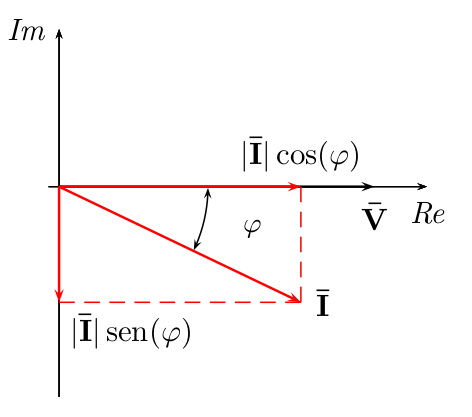
\includegraphics[width=\textwidth]{Imagenes/MarcoTeorico/DiagramaFasorDePotencias.png}}
                        \caption{Diagrama Fasorial.}
                        \label{fig:DiagFasor}
                  \end{subfigure}
                  \hfill
                  \begin{subfigure}[b]{0.5\textwidth}
                        \centering
                        \frame{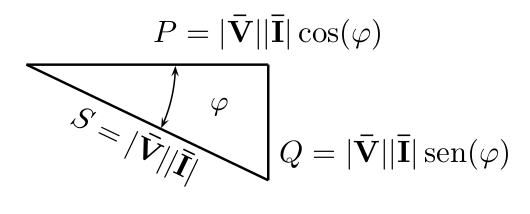
\includegraphics[width=\textwidth]{Imagenes/MarcoTeorico/TrianguloDePotencias.png}}
                        \caption{Triángulo de potencias.}
                        \label{fig:TriangPot}
                  \end{subfigure}
                  \hfill
                  \caption{Obtención del triangulo de potencias.}
                  \label{fig:ObtDeTriagDePot}
               \end{figure}
          
         \subsubsection{Factor de potencia}
         
         El \textbf{factor de potencia} (\textbf{fp}), se lo puede definir como la relación que
               existe entre la energía que es aprovechada, capaz de realizar un trabajo, y la 
               energía total del sistema disponible.
               Dichas energías se relacionan, directamente con la potencia activa (P) y 
               la potencia aparente (S) 
               \begin{equation}
               fp = \frac{W_p}{W_s} = \frac{P}{S} = \dfrac{V I \cos(\varphi)}{V I} \notag \\
                        \hspace{20pt} \therefore \hspace{20pt} \boxed{fp = \cos(\varphi)}~.\label{eqn:fpFinal} 
               \end{equation}

               El factor de potencia, es un valor adimensional que indica 
               el \textbf{rendimiento de un sistema}, es decir, qué parte de la energía disponible 
               se transforma en trabajo. Dicho valor es un número comprendido entre 0 y 1, 
               donde 0 indica que un sistema es \textbf{puramente reactivo}, lo cual quiere 
               decir que toda la energía disponible en él retorna a la fuente en cada ciclo. 
               En el caso de un $fp = 1$ el sistema es \textbf{puramente resistivo},
               es decir, toda la energía disponible en él es consumida por una carga
               transformándose en trabajo.

               En la práctica, se busca un fp lo más
               cercano a 1 para aprovechar al máximo la energía. En caso de no tener un valor
               cercano a la unidad, se realiza lo que se conoce como \textit{corrección de
               factor de potencia}, el cual se explica en la siguiente sección.
               El factor de potencia, al igual que las potencias reactivas, es expresado en 
               términos de \textit{adelanto}, para sistemas de carácter inductivo, o 
               \textit{atraso de fase}, para sistemas de carácter capacitivo.

            \subsubsection{Corrección del factor de potencia}
               
               Como se menciono anteriormente, en los sistemas se busca un factor de potencia 
               lo mas cercano a uno debido a que la \textbf{la energía que es transportada 
               y no se consume produce pérdidas}, por ende, entre mas cercano sea el valor a 
               la unidad las perdidas serán mínimas en el sistema, pero en caso de ser mas alejado 
               al valor unitario, se producirá mayores perdidas en el mismo, debiendo realizar
               una \textbf{corrección del factor de potencia}.

               Dicha corrección se logra, \textbf{conectando cargas reactivas en paralelo, 
               de carácter contrario al que posee el sistema}, de esta manera no se modifica 
               la tensión aplicada en el mismo. El calculo de corrección es realizado en base 
               al \textit{factor de potencia deseado}.
               
               Para la ejecución del trabajo practico, se tiene en cuenta la corrección del 
               fp para una carga inductiva mediante el siguiente planteamiento  
               \begin{align}
                  \intertext{Partiendo de un factor de potencia inicial (\(fp_0\)) a un factor
                  de potencia final (\(fp_f\)) }
                  fp_0  &= \cos(\varphi_0) \hspace{10pt} y \hspace{10pt} fp_f = \cos(\varphi_f) \ , \notag \\
                  \intertext{considerando ambos en atraso para compensar el sistema se 
                  conecta una carga capacitiva de valor (\(Q_C\))}
                  Q_f   &= Q_0 - Q_C \rightarrow Q_C = Q_0 - Q_f  \ , \notag \\
                  \intertext{reemplazando las potencias reactivas como indica la ecuación~(\ref{eqn:PotReacTot})}
                  Q_C   &= V\cdot I_0\cdot \sin(\varphi_0) - V\cdot I_f\cdot \sin(\varphi_f) \ , \notag \\ 
                  Q_C   &= V\cdot I_0\cdot \cos(\varphi_0)\cdot \tan(\varphi_0)  - V\cdot I_f\cdot \cos(\varphi_f)\cdot \tan(\varphi_f) \ , \notag \\
                  \intertext{como la potencia activa (P) no varia entonces}
                  Q_C   &= P\cdot (\tan(\varphi_0) - \tan(\varphi_f)) \ , \notag \\
                  \intertext{finalmente se puede encontrar la capacidad necesaria para la corrección desde el siguiente despeje}
                  \dfrac{V^{2}}{X_C}   &= V^{2}\cdot \omega C = P\cdot (\tan(\varphi_0) - \tan(\varphi_f))  \ , \notag
               \end{align}

                  \begin{equation}
                     \boxed{C = \dfrac{P\cdot (\tan(\varphi_0) - \tan(\varphi_f))}{V^{2}\cdot \omega}}~. \label{eqn:CorrecFp}
                  \end{equation}

      

               
               



							












